\chapter{Conceptual Framework} % Main chapter title

\label{Chapter:ConceptualFramework}

This section of the report opens with an overview of urban agriculture and ends with a conceptual framework for sustainable city.

\section{Overview of urban agriculture}

The Food and Agricultural Organization \cite{FAO2003} defines urban agriculture as any production in the home or plots in an urban area. Central to this definition is the understanding that urban agriculture assumes the nature of farming and gardening in rural areas \cite{Opitz2016}. Whether to consider peri-urban agriculture as part of urban agriculture or not is a subject that remains unresolved in the conventional literature. While some scholars and organisations limit their description of urban agriculture to only gardens and farms within the inner city \cite{NewYorkN.Y..DepartmentofParksandRecreation.2010}, others describe it to include agricultural activities in the peri-urban areas \cite{Mok2014}. Thebo, Drechsel, and Lambin \cite{Thebo2014} make a clear distinction between urban agriculture and peri-urban agriculture based on geographical location. The authors indicate that peri-urban agricultural activities take places within a buffer of 10 to 20 km of the urban geographic boundary. Based on this distinction, the present study focuses on only agricultural activities that take place within an urban geographical boundary or is within 10 km range from a city's core. The work of Ayambire et al. \cite{Ayambire2019} gives a detailed distinction between urban and peri-urban agriculture.

The purpose of urban agriculture differs between cities in the global south and those in the global north. In the latter, people farm typically for recreational or aesthetic reasons although farming for household food supply becomes pervasive during economic meltdowns \cite{McClintock2010}. In the former, farming is mainly to satisfy household food needs and for other commercial reasons \cite{Amponsah2016, McClintock2010}. Typically, households in the cities in the global south farm on undeveloped lands, marginal lands and community plots mainly for food for household consumption whereas empty spaces of post-industrial landscapes are being used for agricultural purposes. Rooftops, balconies and more recently vacant lots, road medians, and parks are used for agricultural purposes in the cities in the global north \cite{McClintock2010}. In this context, urban agriculture is used in the present study to typify crop farming done through community gardens, allotments, backyard gardens and rooftop gardens.

\section{Conceptualising a sustainable city}

The concept of sustainable cities has its roots in the United Nations World Commission on Environment and Development's (UNWCED) idea of sustainable development. The UNWCED summarised sustainable development as meeting the needs of the present generation without compromising the ability of future generations to meet their own needs. The concept has been a standard to strive for in many areas of human activity. It is a normative concept that determines theway humans should act towards nature, as well as the way they should be responsible towards one another and future generations \cite{Yigitcanlar2015}. However, Lew, Ng, and Ni \cite{Lew2016} suggest that numerous definitions of sustainability and sustainable development are sometimes sloppy, vague and narrow. This is partly due to the varied understanding of sustainable development and the numerous semantics in the institutional, ideological and academic definitions of sustainability \cite{Mebratu1998}. For instance, environmental economists believe in economic reductionism by undervaluing ecological goods while social ecologist is reductionist-holistic by focusing on the domination of people and nature. These believes translate into their conception of sustainability and sustainable development. Mebratu \cite{Mebratu1998}, therefore, concludes from the varied conceptions particularly on the cosmic perceptions about the separate existence of nature, economy and society, are problematic for sustainability research. Again, the conceptual understanding and perception of the environment (which comprises living and non-living things) and ecology (which refers to the relationship between living organisms and their environment) as synonymous has affected and continues to affect the conceptual understandings of sustainable development. These can undermine the understanding of a sustainable city since they are intertwined. For clarity, this study's focus on sustainable development considers its tripartite dimension (economic, social and environmental).

In recent times, the sustainable city concept has assumed prominence. This is evident in the Sustainable Development Goal [SDG] 11, which is “to make cities and human settlements inclusive, safe, resilient and sustainable”. The concept's growing prominence is fuelled by rapid urbanisation of the world and the associated effects on environmental quality. The implication is that sustainability should be a crucial objective every development endeavour should strive to achieve. In this regard, the primary goal of urban development should be to make cities and their ecosystems healthy and sustainable \cite{Hiremath2013}. However, the discourse on urban development and urban sustainability has resulted in a plethora of studies equating the sustainable city concept to the new vision of a compact city. This seems to be a conceptual contention like the definition of sustainable development.

The main idea behind the compact city concept is to have a city that is energy-efficient and less polluting because of the proximity of houses to the market centres, shops and work places. The focus is on compactness, which will result in less travel, efficient use of public transportation and ultimately reduce emissions \cite{Abdullahi2015}. Typically, compact cities have less space for green-infrastructure due to the inherent physical and institutional obstacles that limit the quantity and quality of amenity vegetation. Studies have also shown that compactness can have adverse effects on domestic living space, affordable housing, and increased crime levels \cite{Liu2017}. These effects are contrary to the principles of a sustainable city, which emphasise a balance among economic development, environmental protection, and equity in income, employment, shelter, basic services, social infrastructure and transportation \cite{Hiremath}. In this regard, we do not use a compact city interchangeably with a sustainable city in the present study.

The confusion between sustainable city and compact city prompted the authors of this study to provide a clear and comprehensive picture  of the meaning of a sustainable city. As stated earlier, the nuanced conception of sustainable development affects the meaning of a sustainable city. This results in the concentration of indicators that reflect a limited number of dimensions \cite{Tanguay2010}. However, Hellstro \cite{Hellstrom2000}, concludes that it would be unfeasible to try to compile all indicators from all available databases. Therefore, scholars tend to specify on some criteria/indicators based on the focus of their studies and their ideological orientations. For instance, Hellstro \cite{Hellstrom2000} proposed a six study-specific criteria for measuring sustainable urban water management. These criteria are: a) health and hygiene, b) cultural contribution, c) spreading of toxic compounds to water and soil, d) use of natural resources, e) cost benefits, and f) functional risk. The criteria are study-specific and not crosscutting. Many other scholars and organisations use a variety of criteria to define sustainable cities (see: Green City Index, Global City Indicators Facility and the Global Compact Cities Circles of Sustainability). The nuances in the sustainable city indicators are attributable to varied conceptual understanding of a sustainable city discussed above \cite{Huang2015}.

Models and indices are also backed by conceptual views. As such, there is the need to try to complement the strengths and weaknesses of several indicator-sets to derive a more robust and comprehensive model for measuring sustainable city. The use of indicators is also relevant because they provide a much more detailed and quantitative way of measuring the sustainability of a city. Therefore, in this report we review some of the existing models (the Green City Index, Global City Indicators Facility and the Global Compact Cities Circles of Sustainability) to develop a framework that adequately identifies the indicators for a sustainable city. This framework serves as the basis for the discussion of the role of urban agriculture in sustaining cities.

\subsection{The Green City Index}

The Green City Index is regarded as one of the robust models for the identification of a sustainable city \cite{Huang2015}. It comprises 30 indicators, which are grouped under eight categories. These categories are a) environmental governance, b) carbon dioxide (CO2), c) buildings, d) transport, e) water, f) waste and land use, g) energy and h) air quality (refer to Appendix \ref{AppendixA}). The strength of this model lies is its ability to be applied in several geographical contexts. The index has been the basis for the following reports: African Green City Index, Asian Green City Index, European Green City Index, German Green City Index, Latin American Green City Index, and U.S. and Canada Green City Index \cite{Huang2015}. The wide application of the model, its comprehensiveness and attribute as a “strong sustainability indicator” Huang et al. \cite{Huang2015}, were the main reasons for considering it in this paper.

Furthermore, there are some inherent linkages among the suggested indicators. One indicator has effects on the outcome of another. For instance, the indicators on carbon dioxide (CO2), which aims to reduce emissions, are directly linked to the indicators on transportation and air quality. The use of non-car transportation and increased use of green transport will most likely result in the improvement of air quality. This can also lead to the strengthening and sustenance of a green action plan. Again, the indicators on energy are directly linked to the indicators on buildings. The management of energy consumption and the increase in the use of renewable energy are most likely to translate in energy efficient buildings if used in those structures.

\subsection{Global City Indicators Facility}

Unlike the Green City Index, the Global City Indicators Facility attempts to cover all aspects of urban life, with significant emphasis on economic and social measures of sustainability (refer Appendix \ref{AppendixB}). The model conceptualises a sustainable city based on strong economic and social structures. The Global City Indicators Facility was created by the World Bank, working with the Japanese Trust Fund. Compared with the Green City Index, its weakness lies in the limited focus on pollution or air quality, CO2 emissions, clean and renewable energy consumption and environmental governance. However, if cities consider indicators on wastewater, water and particulate matter emissions as suggested in the Global City Indicators Facility, they may accrue direct and external benefits to capture all the environmental indicators suggested by the Green City Index. In addition, the Global City Indicators Facility was designed to focus on cities with over 100,000 inhabitants and lacks a standardisation, which makes it difficult for cities to share best practices and learn from each other \cite{Mccarney2009}. However, this does not dispute its importance in the sustainable city discourse.

In another vein, the Green City Index and the Global City Indicators Facility agree on the use of specific indicators such as particulate matter concentration, solid waste, transportation, wastewater, water consumption and energy. However, they do not cover aspects of embodiment and enough food and flora and fauna. These are essential requirements for sustainable cities \cite{Ackerman2014, Opitz2016, Specht2014}. The implication is that the Green City Index and the Global City Indicators Facility complement each other to identify a robust set of indicators to measure the sustainability of cities. The weaknesses in these models and the earlier contentions in the literature on compact cities and sustainability precipitated the review of the Global Compact Cities Circles of Sustainability.

\subsection{Global Compact Cities Circles of Sustainability}

The Global Compact Cities Circles of Sustainability is a method used for assessing the sustainability and for managing projects directed at socially sustainable outcomes. It has been used by several cities such as Johannesburg, Melbourne, New Delhi, São Paulo and Tehran and by several organisations such as the UN Global Compact Cities Programme, World Vision and Save the Children to understand and support sustainability efforts (KPMG International). It is based on 28 indicators (refer to Appendix \ref{AppendixC}), which are subdivided into four broad categories. These categories are politics, culture, economics and ecology. A scale of critical, being the least, and vibrant, being the best, is used alongside the indicators to rank development efforts.

The inadequacies of the Green City Index and the Global City Indicator Facility in not providing for embodiment, sufficient food and flora and fauna have been covered by the Global Compact Cities Circles of Sustainability. The strength of this index is its global list of indicators as well as its suitability for different countries. An analysis of the Global Compact Cities Circles of Sustainability shows some similarities with the Green City Index and Global City Indicators Facility in terms of the considerations they give to health, education, gender, technology, infrastructure, waste, water and air. Again, the indicators under the Global Compact Cities Circles of Sustainability are complementary. For instance, actions targeted at reducing emissions and waste are more likely to improve the habitat, settlements, recreation, identity and organisation of an area. However, the Global Compact Cities Circles of Sustainability, unlike the Green City Index and the Global City Indicators Facility, does not cover into details the aspects of environment, energy management and civic engagement.

Relevant as these and many other models (such as the Improvement and Efficiency Social Enterprise (IESE) Cities in Motion Index, Gross National Happiness Index and Sustainable Society Index) are in the measurement of the sustainability of a city, the indicators used to measure a city's sustainability vary. This is evident in the observed differences in indicators among the three models covered in this study. This is because the way systems and a city function depend on information flows within them (Meadows, Randers, \& Meadows, 2004). Therefore, choosing which indicators to measure is a crucial determinant of the behaviour of a system or city (Meadows, 1998). Due to this, some suggestions have been made on how to measure a sustainable city since all the indicators are not fixed and applicable in all places and situations. For instance, Tanguay et al. (2010) suggest a method of survey-based selection strategy for Sustainable Development Indicators (SuBSelec). Here, researchers must: a) choose the most cited indicators, b) cover the components of sustainable development and the pertinent predetermined categories and c) choose the simplest sustainability indicators to facilitate data collection, understanding and dissemination. Furthermore, Olsson, T., Aalbu, and Bradley \cite{Olsson2004} suggests the need to make sure selected indicators are: a) relevant to decision making, b) clear in value, c) adequate in scope, d) feasible, e) simple, f) adequately communicated, g) democratic, h) multidimensional, i) distributional, j) forward looking, k) physical, and l) comparable. However, Olsson et al. \cite{Olsson2004}, recognised the difficulties in indicators meeting all the above listed criteria; thus, concluded that the criteria should serve as a guide not a standard in selecting the most applicable.

The criteria presented by scholars (such as: Olsson et al. \cite{Olsson2004} and Tanguay et al. \cite{Tanguay2010}) as well as the suggestion by Hellstro \cite{Hellstrom2000} served as a guide in selecting the indicators for this study. For this reason, the paper presents a framework that merges the indicators for measuring a sustainable city to cover the economic, social and environmental dimensions of a city. The merged framework (Fig. \ref{fig:sustainableCityFramework}) presents the indicators that were used to assess the nexus between urban agricultural and sustainable cities. Overlaps were addressed by taking only one indicator. This however underscores the strength of the indicators in question.

%\begin{figure}[th]
%\centering
%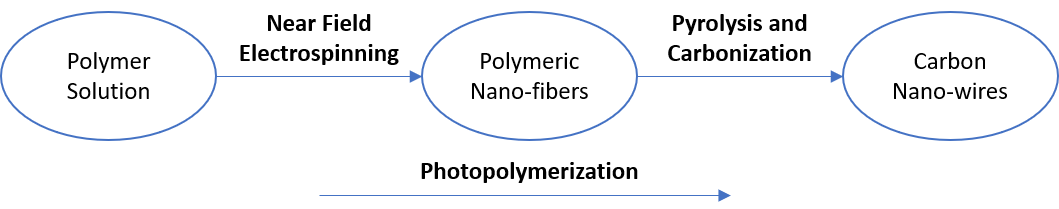
\includegraphics[width=0.95\textwidth]{./Figures/FabricationProcess.png}
%\decoRule
%\caption[Carbon Nano-wires Fabrication Process]{Fabrication process of carbon nano-wires to achieve through the proposed dissertation.}
%\label{fig:fabricationFlowChart}
%\end{figure}

%\begin{equation}
%\left(\tau _t^e-\frac{\tau _n^e \text{dr}}{\text{dz}}\right) 2 \pi  r+\frac{d \left(\pi  r^2
%   \left(\tau _{\text{zz}}-p\right)\right)}{\text{dz}}+\frac{\gamma  \text{dr} 2 \pi  r}{r
%   \text{dz}}+\rho  g \pi  r^2=\frac{d \left(\rho  \pi  r^2 v^2\right)}{\text{dz}}
%\label{eq:linearMomentum}
%\end{equation}